\Chapter{Beam Line Design}\label{chp:4}%________________________________


\Section{Introduction}

Independent staging requires two drive beam lines, with routing of bunch trains via a kicker and septum, 
see Figure \ref{fig:full-staging}. The kicker and septum must direct the beam to a dipole, 
that will straighten the beam trajectory to travel parallel to the original beam path. 
In this configuration the two drive beam lines will be parallel to each other after the dipole.
Several quadrupoles are required to control the beam size, and deliver the desired beam parameters
at the small aperture of the PETS decelerating structure. 
This includes a small transverse size of the beam to allow 100\% transmission, 
and a small bunch length to maximize power extraction from the PETS.
Spectrometer magnets are used to measure the energy of the beam at the end of the beam lines.
This second independent beam line design has been completed. 
So far, installation and testing of the kicker has been done.  
The remaining components have been specified, and several are now ready for installation (i.e. septum, quadrupoles, dipoles).
\begin{figure}
		\begin{center}
		\begin{tikzpicture}[scale=\textwidth/35cm, text=black]
		%\begin{tikzpicture}[scale=0.5, text=black]
		\input{./images/full_staging.tex}
		\end{tikzpicture}
	\end{center}
\caption{The arrows indicate what direction the beams travels.
	The guns are located at opposite ends of the bunker and 
	the propagation direction of the beam lines are opposing.
	PETS stands for Power Extraction and Transfer Structure, and ACC stands for Accelerating structure. 
	The subscript on each structure refers to which stage the structures belong to (first or second). 
	The drive line has six accelerating cavities with a maximum beam energy of \SI{70}{MeV}. 
	The witness line has one accelerating cavity with a maximum beam energy of \SI{15}{MeV}.}
\label{fig:full-staging}
\end{figure}

A kicker design from Indiana University (IU) was used as a base line to design a kicker specific to the
requirements at the AWA. The gap and plate length had to be determined based the beam energy, 
readily available equipment, and mechanical constraints in the AWA tunnel. 
After a design was set, the kicker was fabricated.
Two vacuum tests were performed to verify the fabrication process was successful.
The electronics group at the Advanced Photon Source (APS) provided equipment and helped perform these tests.
The tests included a high voltage (HV) test and Time Domain Reflectometer (TDR) measurement.
Both tests were intended to verify the electrical properties of the kicker were acceptable for operation at HV.
After these tests, the kicker was installed and tested with low and high charge beams. 
The kick was found to be linear with respect to the voltage of the pulser.  
The angle was slightly lower than the simulation result, probably due to reflections at the
connection between the cables and kicker plates. 
The septum design was specified based on simulation work and the kicker angle.
The magnet design was completed at the Institute of Modern Physics (IMP), 
where it was also fabricated. 

The beam line optics also had to be determined and optimized.
The optics include four quadrupoles after the accelerating cavities, 
two quadrupoles on the bent beam line, and three focusing quadrupoles
before the PETS structure.
A point to point matrix calculation was done to ensure that transport of the
beam was possible through the desired kicker gap.  This was followed by an optimization 
performed using the OPAL code and a built-in genetic algorithm. 
There were optimization results in several optics scenarios that can transport 
the beam through the PETS with 100\% transmission.  

This chapter will start with a discussion of the design considerations for the kicker modification for the AWA facility.  
This is followed by a description of the hardware tests done before the kicker installation.  
Simulations relevant to the kicker design will be presented, and compared to beam measurement results.  
The chosen optics design based on the optimization studies will then be presented.


\Section{Kicker Design Theory} \label{theory}

A fast rise time kicker is needed to separate the 
bunch trains supplied by the drive gun.  When the kicker is on, 
bunches passing though it are deflected into an alternate beam line by the kicker field.
The spacing between bunch trains is on the order of nanoseconds; 
it must be long enough to allow the kicker to reach full field before the arrival of the second bunch train, 
and also depends on the layout of the beam lines and laser timing.  
The drive beam and the accelerated `witness' beam must be synchronized so that the 
acceleration field is maximum when the witness beam arrives at the accelerating structure.
Magnetic options for transverse bunch train separation, 
such as a dipole, were disqualified due to their slow rise times 

Borrowing from a successful neighbor, a design implemented by Indiana University (IU) \cite{iukicker}
was adapted to fit the TBA requirements at the AWA. Redesign required consideration
of the length and gap between the kicker plates. Both are key parameters that determine 
what angle the beam will be deflected. Longer plates result in the beam traveling 
in the electromagnetic field for a longer time yielding a larger beam deflection angle. 
A smaller gap increases the field intensity for a given voltage (similar to a parallel plate 
capacitor), increasing the beam deflection angle. 


The kicker is essentially a parallel plate waveguide. 
A $\pm$\SI{30}{kV} power supply can be used to induce a maximum of \SI{60}{kV} potential difference 
across the plates. Each plate will be terminated in a 50 $\Omega$ load.  
The combination of the two plates will result in a static TEM mode 
between the plates. The electric field, $E_x$, and magnetic field, $B_y$,
can be derived from the voltage or current. The electric field, $E_x$, due to a potential, V, is: 
\begin{equation}
E_x=\frac{V}{h}
\end{equation}

where h is the gap height. From Maxwell's equations, we know that the electric and magnetic 
field are related by the speed of light, c, in the case of plane and TEM waves \cite{pozar}. 
From this we can find the magnetic field induced between the plates: 
\begin{equation}
B_y=\frac{E_x}{c}
\label{Bv}
\end{equation}
The electrons are traveling at nearly the speed of light, $c$, and move through the kicker on a 
trajectory perpendicular to the fields.  Plugging Equation \ref{Bv} into the Lorentz force equation, 
it is shown that the force exerted on a charge, q, 
from the electric and magnetic fields of the TEM mode are equal. 
\begin{equation}
F=q\,(E_x+v\times B_y)
\end{equation}
\begin{equation}
	F = q \,\left(E_x+c\times \frac{E_x}{c}\right)
\end{equation}

Since the force due to the electric field is equal and oriented in the same direction as the force due to the magnetic field, 
the total kick is twice that from either field alone.  
The angle induced by electric and magnetic fields has been calculated in \cite{iukicker, Wiedemann}
and is rewritten in the following terms:  
\begin{equation}
\theta_E= \frac{V\,L}{h\,T}
\end{equation}
\begin{equation}
\theta_B= \frac{B\,L}{B\rho}
\end{equation}
Where L is the plate length, and T is the kinetic energy of the beam. 
Rigidity, or $B\rho$, is a common accelerator physics term that can be found in text such as Wiedemann \cite{Wiedemann}. 
It is a convenient way to relate the magnetic field and trajectory of an energetic beam traveling through that field.
\begin{equation}
	B\rho=3.33564\,\,T\, \text{[GeV-Tesla]}
\end{equation} 
For a constant magnetic field, as the beam energy increases, the angle decreases. 
The beam is considered "rigid" at higher energies, 
and requires stronger magnetic fields to achieve the same angle, or bending radius ($\rho$).

Using the definitions above, the total angle provided by the kicker is then: 
\begin{equation}
\theta_k = \theta_{total}= \theta_E+\theta_B=2\theta_E=2\theta_B
\end{equation}
We can also calculate the expected deflection, or x offset after the kicker 
using geometry in Figure~\ref{fig:kicker-geometry}, and the expected angle of deflection. 
\begin{figure*}
	\begin{center}		
		\centering
		\begin{tikzpicture}[scale=0.7]
		\node (fig1) at (0,0)
		{\includegraphics[width=0.75\textwidth]{./images/xoffset_geometry}};
		\node[fill=white, inner sep=2pt] (txt2) at (-2.25,7.5) {L};
		\node[fill=white, inner sep=2pt] (txt2) at (-5,-4.5) {$\theta_k$};
		\node[fill=white, inner sep=2pt] (txt2) at (-6.5,5.5) {$\Delta x$};
		\node[fill=white, inner sep=2pt] (txt2) at (-6.5,0) {$x$};
		\node[fill=white, inner sep=2pt] (txt2) at (-2,3) {Beam Direction};
		\node[fill=white, inner sep=2pt] (txt2) at (-1.5,-2) {$\rho$};
		\node[fill=white, inner sep=2pt] (txt2) at (2,2) {$\theta_k$};
		\end{tikzpicture}
	\end{center} 
	\caption{Simplified drawing of beam trajectory through the kicker.
	Where L is the length of the kicker, $\Delta x$ is the beam offset at the exit of the kicker, 
	$\rho$ is the bending radius, and $\theta_k$ is the kicker angle. }
	\label{fig:kicker-geometry}
\end{figure*}
\begin{equation}
\rho = \Delta x + x 
\end{equation}
\begin{equation}
	\Delta x = \rho - \rho \cos \theta_k
\end{equation}
\begin{equation}
	\triangle x = \left(1-\cos\theta_{k}\right)\rho
	\label{eq:kx}
\end{equation}
Where $\rho$, is the bending radius, $\Delta x$ is the beam offset at the exit of the kicker, 
and $\theta_{k}$ was is the total angle provided by the kicker. 

From these equations, we relate the design parameters gap height, length of the plates, and 
the kinetic energy of the beam. Next, further beam line considerations were included 
to narrow down what angle the kicker needed to supply. 
The largest drive beam energy achievable at the AWA is \SI{75}{MeV}. 
Therefore the kinetic energy of the beam, T, was set as a constant.
Next mechanical constraints were considered. The two drive beam lines need to be separated
by at least \SI{0.5}{m} so that magnets (quadrupoles and dipoles) can fit on each 
beam line without competing for transverse space. 
\begin{figure*}
		\begin{center}		
		\begin{tikzpicture}[scale=0.7]
		\node (fig1) at (0,0)
		{\includegraphics[width=1\textwidth]{./images/tba_geometry}};
		\node[fill=white, inner sep=2pt] (txt2) at (-5,1.3) {$\theta_k$};
		\node[fill=white, inner sep=2pt] (txt2) at (0.2,0.3) {$\theta_s$};
		\node[fill=white, inner sep=2pt] (txt2) at (5,2.5) {Beam Direction};
		\node[fill=white, inner sep=2pt] (txt2) at (5.2,0) {0.5 m};
		\node[fill=white, inner sep=2pt] (txt2) at (2,-1.5) {$\theta_d$};
		\end{tikzpicture}
		\end{center} 
	\caption{Simplified drawing of the TBA layout. 
			The angle provided by the kicker, $\theta_k$, plus the angle provided by the septum, $\theta_s$,
		    must be less than or equal to $20^\circ$.
			The two beam lines must also be at least \SI{0.5}{m} apart.}\label{fig:triangle}
\end{figure*}

Using geometry as shown in Figure \ref{fig:triangle}, an upper limit on the 
combined kicker and septum angle ($\theta_k+\theta_s$) is based on the existing dipoles at the AWA.
The maximum dipole bend angle, $\theta_d$, is $20^\circ$. 
Therefore, $\theta_{total}$  must be less than $20^\circ$. 
That way the bent beam line can be straightened out using a standard dipole, 
which is readily available at the AWA. 
It is also safer to design away from the limit of the equipment. 
Therefore a bend angle less than $20^\circ$ is preferred and allows room for tolerance errors. 
This has the added benefit of reducing energy spread. 
If the beam is bent at a smaller angle, less coherent synchrotron radiation (CSR) and energy spread will be induced.

Using the equations from Section \ref{theory}, 
tables were made for different plate lengths giving possible gap, angle, and x offset values for comparison. 
The maximum beam energy was used, \SI{75}{MeV}, and the expected pulsar voltage was used, \SI{35}{kV}.
Kicker lengths of \SI{0.42}{m}, \SI{0.5}{m}, and \SI{0.6}{m} were investigated.
From these calculations, the range of possible kicker angles fell between \SI{1}{^\circ} and \SI{3}{^\circ}.
The longest kicker plate option was investigated further with the understanding that 
a larger kicker angle would shorten the drift distance between the kicker and septum, 
and the results for this configuration are shown in Table \ref{tab:kickparam}.
A shorter drift would mean less divergence in the beam before it reaches the next focusing optic (quadrupole).
\begin{table}%[hbt]
	%   \vspace*{-.5\baselineskip}
	\begin{center}
		\caption{Possible kicker parameters for a \SI{75}{MeV} beam,  
		a pulsar voltage of $\pm$ \SI{35}{kV}, 
		and kicker plate length of \SI{0.6}{m}.}\label{tab:kickparam}
	\rowcolors{2}{blue!15}{white}   
	\begin{tabular}{ccc}
		\toprule
		\toprule
		%\rowcolor{blue!30} 
		\textbf{Plate Gap [mm]} & \textbf{Angle [deg]}  & \textbf{X Offset [mm]} \\ \hline
		%\midrule
		20 & 3.2   & 16.7    \\ %[3pt]
		25 & 2.57  & 13.4  \\ %[3pt]
		30 & 2.14  & 11.1 \\		 
		35 & 1.83  & 9.6	  \\
		40 & 1.6   & 8.4		 \\
		45 & 1.43  & 7.4      \\
		50 & 1.28  & 6.7   \\ \hline
		%\bottomrule
	\end{tabular}	
	\end{center}
\end{table}

Next simulations were done to give an estimation of the beam size at the entrance and exit of the kicker.
Typical operating conditions at the AWA were used: accelerating cavities on crest, buck focusing at \SI{500}{A}, 
matching solenoid at \SI{255}{A}, and quadrupoles nearly in a 1:2:1 configuration with \SI{1.7}{A} and \SI{-3.3}{A}.
These are not optimized running conditions, which gives a good upper bound for how the beam will behave before tuning.
An angle of \SI{2}{^\circ} was chosen, as a reasonable starting point based on the values in Table \ref{tab:kickparam}. 
\begin{figure}
	\begin{center}		
		\begin{tikzpicture}[scale=0.7]
		\node (fig1) at (0,0)
		{\includegraphics[width=0.5\textwidth]{./images/scatter_kicker_entrance}%
		\includegraphics[width=0.5\textwidth]{./images/scatter_kicker_exit}};
		\node[fill=white, inner sep=2pt] (txt2) at (6,-4) {X [mm]};
		\node[fill=white, inner sep=2pt] (txt2) at (-5,-4) {X [mm]};
		\end{tikzpicture}
	\end{center} 
	\caption{Simulation of the transverse size of a \SI{40}{nC} 
			beam at the entrance and exit of proposed kicker configuration.}
	\label{fig:beamsizekicker}
\end{figure}  
The resulting beam sizes were about \SI{15}{mm} to \SI{19}{mm} as shown in Figure \ref{fig:beamsizekicker}. 
This requires that the kicker gap be comfortably larger than \SI{20}{mm}, 
and have room for the beam centroid deflection that the kicker will cause.
The gap needed to be large enough to allow the full width of the beam to pass through while allowing extra room
for the transverse offset of the beam as it exits the kicker. 

At this point, it was clear the gap needed to be larger than \SI{30}{mm}, due to the beam size at \SI{40}{nC}. 
Around this time, it was also learned that the max pulsar was $\pm$ \SI{30}{kV}, not $\pm$ \SI{35}{kV} as expected. 
These two factors would drive the possible kick angle below \SI{2}{^\circ}, if the kicker plates remained the same length.
The next question was whether to push for a larger angle by elongating the kicker plates, 
or whether plate gap values at \SI{40}{mm} and above were sufficient, see Table \ref{tab:kickparam}.
Additional mechanical constraints between the kicker and septum were considered. 
One beam pipe will connect the two and the deflected and undeflected 
beams must travel in the same pipe until reaching the septum.
After the septum, the two beams will separate into their own beam pipes.
This connection piece before the split, is a custom vacuum chamber designed at 
AWA by Scott Doran, and ordered from MDC Vacuum Products. 
The large chamber requires more vacuum pumping than other areas, 
which could complicate installation if the chamber was too long. 
In this regard, a larger angle from the kicker would help by shortening the pipe length between the kicker and septum.
Therefore, it was decided to elongate the kicker plates to accommodate the larger gap width and still achieve \SI{2}{^\circ}.
 \begin{table}%[h!]
	\begin{center}
		\caption{Mechanical constraints for TBA beam line.}
		\label{tab:mechanical}
		\rowcolors{2}{blue!10}{white}   
		\begin{tabular}{lc}
			\toprule
			\toprule
			%\rowcolor{blue!30} 
			\textbf{Simulation Parameter} 	&  \textbf{Value} \\ 
			\midrule
			Distance between kicker and septum	&  \SI{1}{m} \\
			Distance between deflected/undeflected beam pipe in septum	& \SI{100}{mm} \\
			Distance between parallel drive lines	& \SI{0.5}{m} \\
			Beam Energy 				& 65 MV\\ 
			Linac Voltages 				& 24-25 MV \\
			Kicker Angle				& -2$^\circ$ \\
			Septum Angle				& -15$^\circ$\\ 
			\bottomrule
		\end{tabular}
	\end{center}
\end{table}

After a discussion on fabrication techniques and the mechanical constraints in Table~\ref{tab:mechanical}, 
it was noted that the maximum kicker plate length could be \SI{1}{m}. 
It was also determined from measurements in Chapter~\ref{chp:exp}, 
that the beam energy in the TBA configuration is closer to \SI{65}{MeV}, 
rather than the theoretical maximum of \SI{75}{MeV}.
This is a results of asymmetries in the cavities and the distribution of power
between the witness and drive lines.
A new table of voltages and angles was calculated. At this plate length, 
a gap width of \SI{40}{mm} provided roughly \SI{2}{^\circ} of kick again. 
This angle would satisfy the one inch pipe inner diameter spacing in the septum as well. 

For a length of \SI{1}{m}, and gap of \SI{40}{mm}, 
several beam energy and angle scenarios were considered.
As a contingency plan, it was important to consider if the 
beam energy could be lowered to still achieve the desired 
angle and x offset required in the TBA beam line. 
In other words, if the kicker were unable to deliver a \SI{2}{^\circ}
kick for a \SI{65}{MeV}, could the energy be lowered to still achieve
a fully staged TBA demonstration. 
With the pulsar being variable between 18 and 30 kV,
several feasible options were calculated using the equations in Section \ref{theory}, 
and are shown in Figures~\ref{fig:kickerangles} and \ref{fig:kickeroffset}
\begin{figure}%[h]
	\begin{center}
		\includegraphics[width=0.65\textwidth]{./images/AngleVsEnergy}
		\caption{Calculated angle of deflection for \SI{1}{m} long 
		kicker with a gap of \SI{40}{mm} for several beam energies. The target angle is $2^\circ$.}
		\label{fig:kickerangles}
	\end{center}
\end{figure}
\begin{figure}%[h]
	\begin{center}
		\includegraphics[width=0.65\textwidth]{./images/XoffsetVsEnergy}
		\caption{Calculated x offset of the beam after traveling
		through the \SI{1}{m} long kicker with a gap of \SI{40}{mm}.
		The target x offset is about \SI{20}{mm}.}
		\label{fig:kickeroffset}
	\end{center}
\end{figure}
As a double check on the first order calculations in Figures \ref{fig:kickerangles} and \ref{fig:kickeroffset}, 
a PIC simulation was done to estimate the beam 
trajectory in the kicker and septum. 
This work includes rf cavities and space charge effects.
The two estimates match within reason, see Figure \ref{fig:beamtraj}. 
\begin{figure}
	\begin{center}
		\includegraphics[width=0.65\textwidth]{./images/tba_trajectory}
		\caption{Simulation of the transverse offset of a \SI{65}{MeV} beam as 
			it travels through the proposed TBA beam line. 
			Beam is traveling right to left in this simulation. 
			Notice the x offset at the exit of the kicker (\SI{17.5}{m}), 
			is nearly \SI{20}{mm} as predicted in Figure \ref{fig:kickeroffset}.}
		\label{fig:beamtraj}
	\end{center}
\end{figure}

\Section{Preliminary Kicker Tests}

After the design of the kicker was finalized, fabrication began at ANL.
The copper plates and ceramic brackets were fabricated on site at the ANL shops.
High voltage (HV) feedthroughs and cables were purchased from FID GmbH. 
In order to test that the fabrication of the kicker was sound, members of the 
Advanced Photon Source (APS) electronics groups graciously helped perform an 
out of vacuum AC high voltage test. Afterwards they also helped perform and 
analyze a Time Domain Reflectometer (TDR) measurement of the kicker plates
to determine the impedance along the kicker plates, feedthroughs, and cables. 
\begin{figure*}
	\begin{center}		
		\begin{tikzpicture}[scale=0.7]
		\node (fig1) at (0,0)
		{\includegraphics[width=1\textwidth]{./images/kicker}};
		\node[fill=white, inner sep=2pt] (txt2) at (-10,0) {Port 1};
		\node[fill=white, inner sep=2pt] (txt2) at (-5, -5) {Port 3};
		\node[fill=white, inner sep=2pt] (txt2) at (5.5,6) {Port 2};
		\node[fill=white, inner sep=2pt] (txt2) at (10,1) {Port 4};
		\end{tikzpicture}
	\end{center} 
	\caption{CAD drawing of AWA kicker design, courtesy of Scott Doran from AWA.
	Ports are connected the HV cables purchased from FID GmbH. 
	Power is suppled by a pulsar also fabricated by FID GmbH and borrowed from the APS Electronics group.}
\end{figure*}\label{fig:AWAkicker}
\begin{figure}%[h]
	\begin{center}
		\includegraphics[width=0.5\textwidth]{./images/FID_feedthrough1}\includegraphics[width=0.5\textwidth]{./images/FID_feedthrough2}
		\caption{High voltage feedthrough purchased from FID GmbH. Left, connection to the HV cables.
		Right, the in vacuum pin that connects to the copper kicker plates.
	Photos supplied by FID GmBH.}
		\label{fig:feedthroughs}
	\end{center}
\end{figure}
\iffalse
\begin{figure}
	\centering
	\includegraphics[width=0.75\textwidth]{./images/kicker_plates}
	\caption{Inside of kicker vacuum chamber after assembly. }
	\label{fig:kicker-plates}
\end{figure}
\fi

\Subsection{High Voltage Kicker Test}
Two HV tests were performed at the APS. This was done to ensure the electrical connection 
between the feedthroughs and kicker plates were free of shorts. 
The first test consisted of HV applied in increments to ports 3 and 4 on the kicker.  
Ports 1 and 2 were shorted to ground. There was no leakage current up to \SI{8}{kV} RMS.
The second test reversed the set up with 3 and 4 grounded and ports 1 and 2 exposed. 
There was no leakage current up to \SI{9}{kV} RMS, which was the maximum voltage of the test equipment.
Figure~\ref{fig:AWAHVkicker} shows the connection and location of the kicker in the APS Faraday cage.
\begin{figure}%[h]
	\begin{center}
		\includegraphics[width=\textwidth]{./images/kicker1}
		\caption{High voltage test cage at the APS. 
			The kicker was grounded on one side and exposed to high voltage AC power on the other. 
			The Faraday cage was closed during testing. }
		\label{fig:AWAHVkicker}
	\end{center}
\end{figure}


\Subsection{Time Domain Reflectometer Test}
After the HV test was completed, a Time Domain Reflectometer (TDR) measurement was preformed at the APS~\cite{TDR}, 
with the help of C. Y. Yao, A. Brill, X. Sun and C. Jing.
This technique measures reflections along a conductor and gives information about discontinuities in the line being measured. 
This information was used to determine the impedance along the cables, feedthroughs, and plates of the kicker. 
Ideally, the response would be \SI{50}{\ohm} to reduce reflections and resulting power loss. 
The measurements, plotted by C.Y. Yao in Figure \ref{fig:TDR}, show a larger impedance at the feedthrough locations.
Due to resource and time constraints, it was a goal to use off the shelf parts where possible in fabrication of the kicker.
Therefore, the feedthrough mismatch is expected because they were not specifically designed to couple to the plate geometry.
A substantial amount of time and resources were spent to minimize reflections for the APS kickers plotted in Figure \ref{fig:TDR}.
However, that kicker still deviates from \SI{50}{\ohm} near the feedthroughs.
Given this comparison to the kickers fabricated at the APS, C. Y. Yao advised the mismatch we observed was not dangerous to 
the pulsar or cables that would drive the kicker.  
The only negative result is the reduced amount of voltage supplied to the plates, and therefore, a reduction in the kick given to the beam.
	\begin{figure}
		\begin{center}
			\includegraphics[width=0.75\textwidth]{./images/TDR_AWA_kicker}
			
			(a) TDR single mode measurements of the AWA kicker.
		\end{center}
		\begin{center}
		\includegraphics[width=0.75\textwidth]{./images/TDR_APS_kicker}
	
		(b) TDR single mode measurements of an APS kicker.
		\caption{TDR measurements of the impedance of AWA and APS kickers, plotted by C. Y. Yao.
		Single mode refers to the orientation of the measurement. 
		Only one port of the kicker is driven and measured at a time. }\label{fig:TDR}		
		\end{center}
	
	\end{figure}


\Section{Measurement of Beam Deflection}

Once the kicker was installed, measurements were done to verify it worked as designed with beam.  
The voltage was scanned to check for linearity of the beam offset with voltage.  
The beam size and angle of deflection were measured and compared to simulation results.  
Details of the set up, and results of the studies follow.

The kicker was installed in the AWA drive beam line approximately \SI{16.5}{m} downstream of the cathode.
The HV pulsar was located on the roof of the bunker.
During the beam tests the accelerator was operated in TBA-like conditions with machine settings based on simulations 
done to optimize for future TBA runs, see Table~\ref{tab:krunparam}.
 \begin{table}%[h!]
	\begin{center}
		\caption{Beam line configuration when kicker was tested.}
		\label{tab:krunparam}
		\rowcolors{2}{blue!10}{white}   
		\begin{tabular}{lc}
			\toprule
			\toprule
			%\rowcolor{blue!30} 
			\textbf{Parameter} 		&  \textbf{Value} \\ 
			\midrule
			Charge					&  \SI{30}{nC} \\
			Laser dimension in x    &  \SI{19}{mm} \\
			Laser dimension in y    &  \SI{16}{mm} \\
			Buck Focusing Solenoid	& \SI{550}{A} \\
			Matching Solenoid		& \SI{200}{A} \\
			Quad 1					& \SI{0}{A}  \\
			Quad 2					& \SI{-1.53}{A}  \\
			Quad 3					& \SI{3.08}{A}  \\
			Quad 4					& \SI{-1.53}{A}  \\
			Cavity phases   		& -20$^\circ$ \\
			Beam Energy 				& 65 MV\\ 
			\bottomrule
		\end{tabular}
	\end{center}
\end{table}
All accelerating cavities were operated at \SI{-20}{^\circ} off crest to minimize energy spread.
A simplified experimental setup is shown in Figure~\ref{fig:kyag}
\iffalse
\begin{figure*}
	\begin{center}		
		\begin{tikzpicture}[scale=0.7]
		\node (fig1) at (0,0)
		{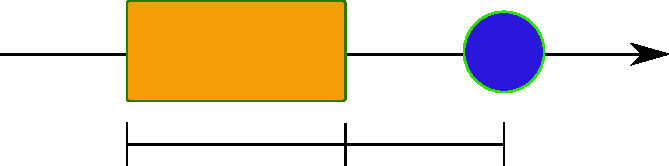
\includegraphics[width=0.5\textwidth]{./images/kicker_yag}};
		\node[fill=white, inner sep=2pt] (txt2) at (-1.5,2) {Kicker};
		\node[fill=white, inner sep=2pt] (txt2) at (-1.5,-1.5) {\SI{1}{m}};
		\node[fill=white, inner sep=2pt] (txt2) at (6.5,-0.75) {Beam Direction};
		\node[fill=white, inner sep=2pt] (txt2) at (3,2) {YAG Screen};
		\node[fill=white, inner sep=2pt] (txt2) at (1.5,-1.5) {\SI{0.28}{m}};
		\end{tikzpicture}
	\end{center} 
	\caption{Simplified drawing of kicker and YAG screen where beam size and offset data 
		was taken. This experimental set up was used to calculate 
		the angle provided by the kicker for a \SI{30}{nC} beam at \SI{65}{MeV}.}\label{fig:kyag}
\end{figure*}
\fi
The centroid position of the beam was measured for several kicker voltages, and a linear fit was performed.
The R value for the fit in Figure \ref{fig:linear} is 0.99704. This shows that the beam offset 
is fairly linear with respect to kicker voltage. 
\begin{figure}
	\centering
	\includegraphics[width=0.75\textwidth]{./images/kicker_linearity}
	\caption{Measured deflection of beam due to kicker at several voltages.}
	\label{fig:linear}
\end{figure}

Using the x offset numbers found in Figure~\ref{fig:linear}, 
the measured angle vs. first order approximations from Section~\ref{theory} can be compared . 
Note the x offset seen on the YAG screen is not solely due to the trajectory in the kicker.
The contributions to the total deflection must be broken into two parts: the deflection of the beam inside the kicker, 
and the position change when the beam is drifting towards the YAG screen after it exits the kicker.
The later part can be approximated as a triangle as shown in Figure~\ref{fig:kicker-geometry}.
Inside the kicker, the trajectory is approximated using Equation~\ref{eq:kx}. 
Combining these two terms, the equation for the x offset seen during the experiment
can be written as:
\begin{equation}
	\Delta x = \Delta x_{kicker} + \Delta x_{drift}
\end{equation}
\begin{equation}
	\Delta x = \left(1-\cos\theta_{k}\right)\rho + L_{drift} \tan \theta_{k}
	\label{eq:kdata}
\end{equation}
Where $\rho$ is the bending radius in the kicker, and $L_{drift}$ is \SI{0.28}{m} as shown in Figure~\ref{fig:kyag}.
Using the small angle approximation, this equation simplifies to:
\begin{equation}
	\Delta x = \rho - \rho \left(1-\frac{\theta^2}{2}\right) + L_{drift} \theta_{k}
\end{equation}
\begin{equation}
	\Delta x = \rho \frac{\theta^2}{2} + L_{drift} \theta_{k}
\end{equation}
Next, $\rho$ is rewritten assuming the the arc length is approximately equal 
to the length of the kicker plates:
\begin{equation}
	\Delta x = \frac{L_{kicker}}{\theta_{k}}\frac{\theta_{k}^2}{2} + L_{drift}\theta_{k}
\end{equation}
\begin{equation}
	\Delta x = \left(\frac{L_{kicker}}{2}+ L_{drift}\right)\theta_{k}
\end{equation}
Where the length of the kicker is \SI{1}{m} and the drift is \SI{0.28}{m}:
\begin{equation}
	\Delta x = \SI{0.78}{m}\,\,\theta_{k}
		\label{eq:kdx}
\end{equation}
In Equation~\ref{eq:kdx}, $\Delta x$, was measured and is the data shown in Figure~\ref{fig:linear}. 
Note, the beam centroid location at kicker voltage $=0$, 
represents the beam location on the YAG screen when the kicker is turned off.
This is used as a reference point to calculate $\Delta x$ at each voltage value
(i.e. $\Delta x_i = x_{vi} - x_{v0}$).
With these $\Delta x$ values, Equation~\ref{eq:kdata} can be rewritten to 
solve for the experimentally achieved angle $\theta_{k}$.

Next the energy measurement was analyzed to determine the beam energy. 
The method described in Chapter \ref{chp:exp} was used, 
and the current measured to bend the beam \SI{15}{^\circ} was about \SI{9}{A}.
This corresponds to an energy of about \SI{65}{MeV} \nrnote{double check w/ Shao}. 
This energy was then used to calculate the ideal angle values vs. kicker voltage.
The are plotted in Figure~\ref{fig:angles} in comparison 
to the ideal values for a \SI{65}{MeV} beam. 
\begin{figure}
	\centering
	\includegraphics[width=0.75\textwidth]{./images/kicker_angle_comparison}
	\caption{Measured angle provided by the kicker at several voltages.  
	These are compared to 1st order calculations for a \SI{65}{MeV} beam.
	Smaller angles are expected in the data due to the reflections
	seen at the feedthroughs in TDR measurements, see Figure~\ref{fig:TDR}.
	Note the calculated values are also smaller than the 
	angles predicted in Figure~\ref{fig:kickerangles}, 
	because the final kicker gap after assembly was \SI{45}{mm}, a little larger
	than the design value of \SI{40}{mm}}
	\label{fig:angles}
\end{figure}

Beam size data on the YAG screen after the kicker was taken, 
see Figure \ref{fig:kickerbeamsize} for examples of this data. 
These measurements were used to calculate the total beam size and 
centroid location of the beam. A combination fit was used to extract 
the beam sizes as described in Section~\ref{sec:beamsize}. 
A Gaussian fit was used for the beam core, and linear fits were used for the tails.
\begin{figure}
	\includegraphics[width=0.5\textwidth]{./images/yag6_kicker_voltage0}%
	\includegraphics[width=0.5\textwidth]{./images/yag6_kicker_voltage18}\\
	\includegraphics[width=0.5\textwidth]{./images/yag6_kicker_voltage20}%
	\includegraphics[width=0.5\textwidth]{./images/yag6_kicker_voltage22}%
	\caption{Examples of beam size data taken during kicker test. 
		Various kicker voltage settings were used and deflection of the beam was observed.}
	\label{fig:kickerbeamsize}
\end{figure}
The kicker slightly increase the beam size in the kicked direction (x), 
but the large discrepancy in the horizontal and vertical beam size can not be attributed to the kicker alone.
If the asymmetries were due to the kicker only, they would not be present when the kicker is off.
Persistence of the asymmetry when the kicker is off (voltage = 0) indicates 
the sources of error is not an intrinsic problem associated with the kicker.
\begin{figure}
	\centering
	\includegraphics[width=0.8\textwidth]{./images/xybeamsizes_high_charge_kicker_scan_angle_asymmetric}
	\caption{Beam size data taken during kicker voltage scan. Asymmetry between the x and y beam sizes
		 is present even when the kicker is off at V = 0. This suggests the asymmetry is not
	     caused by the kicker alone. Scans of the gun voltage showed large impact on the beam sizes
     	 and is probably the source of the majority of the asymmetry in the x and y dimensions.
	 The gun gradient to get the simulation values shown in this figure was \SI{55}{MV/m}.} 
     \label{fig:beamsize}
\end{figure}

There are several possible sources of the asymmetric beam sizes. 
These include the initial laser profile (which was not exactly symmetric
when the data was taken), field strengths in the accelerating cavities, 
and uncertainties in the quadrupoles strengths.
The solenoid field is excluded due to a recent measurement of the magnetic field, 
done by G. Ha and E. Wisniewski at the AWA. 
To check the laser radius contribution, symmetric and asymmetric simulations were done.
The difference in the x beam size in these two cases was only \SI{0.3}{mm} rms. 
Therefore, this is not the major contributing factor.

Next, several gradient values in the gun were simulated. 
This parameter had a strong impact on the beam sizes, with a range of \SI{1.5}{mm} 
in the x direction and \SI{0.3}{mm} in the y direction.
It's clear the field strength and asymmetries in the RF field map 
are strongly affecting the results seen in Figure~\ref{fig:beamsize}.
Details of the simulation set up for these tests can be found in Appendix~\ref{gunsims}.
The gradient that achieved the agreement seen in Figure~\ref{fig:beamsize} was \SI{55}{MV/m}.
This is considerably lower than the reported AWA maximum gradient of \SI{85}{MV/m}.
It is possible that the lower gradient and resulting asymmetric beam size effect is 
distributed in lower gradients for the cavities. 
In other words, perhaps the the gradient in the gun is not that low, but rather
the gradients in the gun and all six linac cavities are slightly lower than expected.

In conclusion, there are several contributing factors to the asymmetries in the beam.
From simulations, the laser radius mismatch contributes an estimated \SI{0.3}{mm} of difference 
between the x and y dimensions. Also in simulation, a difference of about \SI{1.5}{mm} 
is attributed to the gun gradient and asymmetries in the RF fields. 
This is an unexpected and meaningful result for the AWA, and will inform experiments moving forward.
Finally, there is a variance of ~\SI{0.5}{mm} attributed to the kicker through analysis of the 
data shown in Figure~\ref{fig:beamsize}.
Note, these errors are not a major hurdle for TBA experiments, as they can
be mitigated with precise control of the quadrupoles.


\Section{TBA Beam Line}

While  the kicker and septum parameters were defined by the constraints discussed above, 
the optics must be used to address the aperture limits further down stream.
There were three clear goals TBA beam line configuration: 
\begin{itemize}
	\item Achieve 100\% transmission in the PETS
	\item Achieve the smallest bunch length possible
	\item Arrange the beam line for quick and easy installation
\end{itemize}

With the third item addressed partially addressed in Section~\ref{theory}, 
it remained to determine if an optics solution exists that can satisfy the 
first two requirements (transmission and bunch length). 
In the case of bunch length, there was no set goal, but a clear understanding 
that a shorter bunch will generate more power in the PETS structures [ref here].
Regarding transmission, an aperture of \SI{17.6}{mm} exists at the PETS.
This is roughly three times smaller than the rest of the beam line.

As a first check, a point to point matrix calculation was done 
to determine if the beam size could be maintained near the kicker.
Next the information presented in Chapter~\ref{simulations} was used to form the 
base line of further optimization efforts. The genetic algorithm in OPAL
was used to explore and optimize the optics in the TBA beam line.
Solutions were found that meet the requirements listed above.



\Subsection{Point to Point Check}
The effect of a beam line component (such as a dipole, quadrupole, or straight beam pipe) on the phase space coordinates of a particle can be modeled as a matrix operator~\cite{brown,Wiedemann}.  These building blocks may be `stacked' to model the effect of an entire beam line, or section of a beam line, on the coordinates of a  particle.  
These common building blocks were used as a check that the 
beam properties after the first four quadrupoles 
would allow transport through the kicker (see Figure~\ref{fig:full-staging}),
\begin{figure*}
	\begin{center}		
		\begin{tikzpicture}[scale=0.7]
		\node (fig1) at (0,0)
		{\includegraphics[width=0.5\textwidth]{./images/p2p_optics}};
		\node[fill=white, inner sep=2pt] (txt2) at (-4.8,-2) {$f_1$};
		\node[fill=white, inner sep=2pt] (txt2) at (-2.7,-2) {$f_1+f_2$};
		\node[fill=white, inner sep=2pt] (txt2) at (7,0.0) {Beam Direction};
		\node[fill=white, inner sep=2pt] (txt2) at (0,-2) {$f_2+f_3$};
		\node[fill=white, inner sep=2pt] (txt2) at (2.7,-2) {$f_3+f_4$};
		\node[fill=white, inner sep=2pt] (txt2) at (4.7,-2) {$f_4$};
		\end{tikzpicture}
	\end{center} 
	\caption{Simplified drawing of a point to point optics configuration for quadruplet telescope model.}
		\label{fig:p2p}
\end{figure*}
by establishing that the beam size could be maintained near the kicker during transport.  
Four quadruple strengths and the five distances between the quadrupoles are parameters under consideration. 
To reduce the number of variables from ten to four, the drift lengths are set to be sums of focal lengths, as in
the quadruplet telescope module described by K. Brown in \cite{brown}.  
The transfer matrix R, defined as:  
\begin{equation}
	R_q =  R_{d5}  \cdot R_{q4} \cdot   R_{d4} \cdot R_{q3} \cdot R_{d3} \cdot R_{q2} \cdot R_{d2} \cdot R_{q1} \cdot R_{d1} 
\label{kb1}
\end{equation}
where a matrix with the subscript d refers to a drift as defined by,
\begin{equation}
R_{d_i} = 
\begin{bmatrix}
1 & L_i \\
0 & 1
\end{bmatrix}
\end{equation}
and a matrix with subscript q refers to a quadrupole as defined by,
\begin{equation}
R_{q_i} = 
\begin{bmatrix}
1 & 0 \\
\pm \frac{1}{f_i} & 1
\end{bmatrix}
\end{equation}
Substitution and matrix multiplication results in a transfer matrix of the 
the following form for the quadruplet:
\begin{equation}
R_q = 
\begin{bmatrix}
\frac{f_2 f_4}{f_1 f_3} & 0 \\
0 & \frac{f_1 f_3}{f_2 f_4}	
\end{bmatrix}\label{kb2}
\end{equation}
Where $f_1 \ldots f_4$ stand for the focal lengths of each quad before the kicker. 
Due to other experiments in the AWA tunnel, 
the first quadrupole was required to be at least $\SI{3}{m}$ away from the exit of the 
last accelerating cavity in the linac. This gives the initial drift length and value
for $f_1$, see Figure~\ref{fig:p2p}.
To achieve point to point transport of the beam as described in~\cite{brown}, 
we can equate $f_1 = f_4$ and $f_2 = f_3$. This reduces Equation~\ref{kb2} to:
\begin{equation}
R_q =
\begin{bmatrix}
1 & 0 \\
0 & 1	
\end{bmatrix}
\end{equation}
We can further simplify this problem set up by 
assuming $f_1=f_2$. 
Given the total distance, D, available for the
quads in the beam line, \SI{3.8}{m}, and refering to Figure~\ref{fig:p2p}, 
an equation is written to solve for the focal length $f_1$: 
\begin{align}
D = 2 \left(f_1+f_2+f_3+f_4\right)\\
= 4f_1 + 4 f_2 \\
8f_1 = \SI{3.8}{m} \\
f_1 = \SI{0.475}{m}
\end{align}

For completion, the focal length is converted into a field strength 
to determine whether or not this configuration is possible given 
the currently installed hardware at the AWA. 
\begin{equation}
\frac{1}{f} = kl 
\end{equation}
Where $l$ is the quadrupole's effective length, and k is the gradient w.r.t 
the beam energy and magnet strength \cite{Wiedemann}:
\begin{equation}
k = \SI{0.2998}{} \frac{g[\SI{}{T/m}]}{p [\SI{}{GeV/c}]}\label{k}
\end{equation}
The beam energy must also be accounted for with the dimensions of the quadrupole. 
Given an energy of \SI{65}{MeV}, a quadrupole length of \SI{11}{cm}, 
and Equation~\ref{k} we can calculate this configuration would require a 
magnet strength of \SI{\pm4.14}{T/m}. This is feasible considering the 
max strength is \SI{\pm9}{T/m}. This also gives some indication that 
that there should be several possible solutions found during optimization
since the point to point check is not at either extreme of the quadrupole limits.


\iffalse
To determine the effect of this configuration on the beam size and divergence
we compare the sigma matrix before and after the qudrupoles:
\begin{align}
\sigma_1 = R\cdot \sigma_0 \cdot R^T \\
= 
\begin{bmatrix}
1 & 0 \\
0 & 1	
\end{bmatrix}
\begin{bmatrix}
1 & 0 \\
0 & 1	
\end{bmatrix}
\begin{bmatrix}
1 & 0 \\
0 & 1	
\end{bmatrix} \\
=
\begin{bmatrix}
1 & 0 \\
0 & 1	
\end{bmatrix}
\end{align}
\fi

\Section{TBA Beam Line Optics Optimization}\label{failed}
 
With the kicker and septum design set, 
and the basic geometry of the beam line laid out, 
an optimization of the beam line optics was performed.
This was done for two reasons. First, to confirm that solutions 
exist at \SI{40}{nC} where the beam is transmitted 100\% through the PETS structure in the deflected beam line.
Second, from the set of feasible solutions, the optics designs with the smallest bunch lengths should be identified.
These two conditions combined will provide an optics solution that provides the most power output from the PETS structure for acceleration of the witness beam. 

The built in GA in OPAL was again used for these simulations. 
Several rounds of optimizations were tried and many failed for various reasons, 
some of which include:
\begin{itemize}
	\item using too many objectives (7+)
	\item including too many design variables (15+)
	\item over constraint of the objective values (upper bound too small at \SI{0.1}{mm} for beam sizes)
	\item using bad hyper parameters
	\item setting the first optimization point upstream near the linac
\end{itemize}
All iterations can be found in the following repository:
\begin{center}
	\url{https://github.com/nneveu/awa-tba}
\end{center}
which also houses all plotting and simulation scripts used in this chapter.

Some draw backs of using a GA, is that many simulation parameters 
must be decided empirically after trial and error.
This can be computationally expensive, 
and there is no clear guidance on what type of problem set up will be 
best for unique optimization problems such as the beam dynamics in this case.
Luckily, ANL provides excellent computational resources \cite{lcrc}, and
the availability of compute time was not a limiting factor in this work.
\iffalse
Along these lines, hyper parameters were chosen based on four experiments 
with various GA settings.
GA runs with various settings, see Table \ref{tab:ex}. 
It is clear that the hyper parameters in ex-2 and ex-3 are evolving slower in 
comparison to ex-1 and ex-4. 
Much help was received from A. Adelmann in preparing and discussing these tests.
\begin{table}%[h!]
	\begin{center}
		\caption{Input Parameters for initial twenty four hour TBA optimization experiments. 
			The gene mutation probability was equal to the mutation probability (not shown) in all four experiments. 
			The max number of individuals per generation was~80.}
		\label{tab:ex}
		\rowcolors{2}{blue!15}{white}   
		\begin{tabular}{|lccc|}
	%\toprule
		\rowcolor{blue!30} 
				& \thead{Gene Mutation\\Probability} & \thead{Recombination\\Probability} & \thead{Number of completed\\generations} \\ \hline
			ex-1 &  0.1  & 0.9  &  96 \\
			ex-2 &  0.3  & 0.7  &  81 \\
			ex-3 &  0.8  & 0.2  &  53 \\
			ex-4 &  0.01 & 0.09 &  95 \\ \hline
		\end{tabular}
	\end{center}
\end{table}
\fi

\Subsection{Optimization Setup}\label{setup}
The most successful optimization problem to date entailed optimizing the 
3D beam size, transverse momentum, and energy spread at the fifth quarupole on the drive line.
In other words, the first quadrupole between the septum and kicker.
Optimizing at this location helps reduce dispersion by minimizing 
the energy spread before it enters the $15^\circ$ bend that straightens out 
the deflected beam line, see Figure~\ref{fig:full-staging}.
This helps reduce transverse beam size growth in the last dipole.
\begin{table}%[h!]
	\begin{center}
		\caption{Input GA Parameters for large scale TBA optimization runs.}
		\label{tab:opt-tba}
		\rowcolors{2}{blue!10}{white}   
		\begin{tabular}{lc}
			\toprule
			\toprule
			%\rowcolor{blue!30} 
			\textbf{Simulation Parameter} 	&  \textbf{Value} \\ 
			\midrule
			{Number of Objectives}			&  6 \\
			Number of Design Variables		&  8 \\
			Number of Constraints			&  2 \\
			{Gene Mutation Probability} 	&  0.01\\ 
			{Recombination Probability} 	&  0.09 \\
			{Maximum  Generations}			&  200 \\
			{Initial  Population Size}		&  656\\ 
			Cores per Simulation 			&  8 \\
			Total number of cores			& 2,624  \\
			\bottomrule
		\end{tabular}
	\end{center}
\end{table}
In code form, these parameters translate to an OPAL input file that 
can be found in Appendix~\ref{opt-tba-code}.
\begin{table}%[h!]
	\begin{center}
		\caption{\lsnote{Non-varying \sout{Non-varing}} Input Parameters for large scale TBA optimization runs.}
		\label{tab:variables}
		\rowcolors{2}{blue!10}{white}   
		\begin{tabular}{lc}
			\toprule
			\toprule
			%\rowcolor{blue!30} 
			\textbf{Simulation Parameter} 	&  \textbf{Value} \\ 
			\midrule
			Cavity Phases		&  -20$^\circ$ \\
			Laser Radius		& 9 mm \\
			Laser Full Width Half Max	& 10 ps \\
			Gun Voltage 				& 64 MV\\ 
			Linac Voltages 				& 24-25 MV \\
			Kicker Angle				& -2$^\circ$ \\
			Septum Angle				& -15$^\circ$\\ 
			\bottomrule
		\end{tabular}
	\end{center}
\end{table}
The OPAL input file and other files needed to run simulations on the ANL cluster 
can be found in the repository listed above.
Details of how the magnet settings, phases, and element locations defined 
in Table~\ref{tab:variables} are also in the repository.


\Subsection{Optimization Results}
After fourty-eight hours, the optimization run described in Section \ref{setup}
completed and the results were analyzed. 
A Pareto front comparing the trade off between bunch length and energy spread was plotted.  \lsnote{{\it I don't really understand this.  The Pareto front for bunch length and transverse emittance makes sense because 6D emittance is conserved, and there really is a trade off between those parameters.  Bunch length and energy spread make less sense to me, given a specific bunch length, the energy spread should depend on the bucket height.  According to table  4.5, you don't allow anything that should impact the longitudinal parameters to vary, other than solenoid, which could do emittance exchange. These differences in bunch length shown may be due to the transverse emittance and not the momentum spread.}}
\begin{figure}
	\centering
	\includegraphics[width=0.75\textwidth]{./images/dE_vs_zrms_pareto_front_quads_before_Q5}
	\caption{Simulated Pareto front of energy spread vs. bunch length.
	This data was a result of the simulation setup in Section \ref{setup}.}
\label{fig:tba-pareto}
\end{figure}
From Figure~\ref{fig:tba-pareto}, there are not many bunch lengths options.
Only one point is excluded from the plot at \SI{5}{mm}, a region 
not desirable for TBA. The results in the transverse dimension were
more instructive. Two Pareto fronts comparing beam sizes
and momentum in the x and y dimensions are plotted in Figure~\ref{fig:tba-paretoxy}.
As expected the beam sizes in the x dimension are larger 
due to the bending elements. This indicates the x dimension will be the 
limiting factor in areas with tight apertures such as the PETS.  \lsnote{{\it A host of questions arises here as well.  Maybe differences are due to longitudinal trade-offs?   What the final values of variable  parameters for the solutions in your figure, and what are all the beam parameters at every point (longitudinal and transverse)?  On the other hand, varying only quadrupoles cannot affect bunch length, etc. so in this case you are truly optimizing only transverse parameters at a given location - anyway, clarification is needed here.}}
\iftrue
\begin{figure}
	\centering
	\includegraphics[width=0.75\textwidth]{./images/xy_vs_pxy_pareto_front_quads_before_Q5}
	\caption{Simulated Pareto front of beam size vs. momentum.
		This data was a result of the simulation setup in Section \ref{setup}.}
	\label{fig:tba-paretoxy}
\end{figure}
\fi
Note the two curves in Figure~\ref{fig:tba-paretoxy}, may not represent the same 
design variables for a point to point comparison. A Pareto analysis always 
chooses the best points w.r.t the objectives chosen. This guarantees no 
relationship between all objectives. 
For example, the smallest beam size in y, at less than \SI{0.35}{mm} on Figure~\ref{fig:tba-paretoxy}, 
may not have the \lsnote{same input parameter settings for the} matching solenoid or quad strengths, as the smallest x position 
at a little over \SI{2.5}{mm}. In other words, the best optics scenario for the x dimension
may or may not be the best optics scenario for the y dimension. 

With this in mind, the Pareto front was re-plotted in Figure~\ref{fig:tba-paretoxonly} 
with one key difference. The y values were forced to coincide with the same 
design variables used in the x dimension. 
Now a true point to point comparison is possible in this plot.
We chose the \lsnote{values of momentum spread to coincide with small horizontal beam size, since this was more difficult to achieve than small vertical beam size, see \sout{x dimension to be the determining plot, 
due to it's clear limitations in comparison to the y dimensions in}} Figure~\ref{fig:tba-paretoxy}. 
\nrnote{the sentences above are awkward, not sure how to word this} 
\iftrue
\begin{figure}
	\centering
	\includegraphics[width=0.75\textwidth]{./images/xonly_pareto_front_quads_before_Q5}
	\caption{Simulated Pareto front of beam size vs. momentum.
		Adjusted to force y beam sizes to correspond to same design variables 
		as the x beam sizes.
		This data was a result of the simulation setup in Section \ref{setup}.}
	\label{fig:tba-paretoxonly}
\end{figure}
\fi
The momentum variance in Figure~\ref{fig:tba-paretoxonly} is small in comparison to 
the beam size variance. Therefore, design variable values resulting in a smaller 
beam size were give higher priority. Table~\ref{tab:designopt}, shows a summary of 
design variables for the four smallest beam sizes.
\begin{table}%[h!]
	\begin{center}
		\caption{Input Parameters for large scale TBA optimization runs.
		Points are numbered for later reference.}
		\label{tab:designopt}
		\rowcolors{2}{blue!10}{white}   
		\begin{tabular}{lcccc}
			\toprule
			\toprule
			%\rowcolor{blue!30} 
			\textbf{Simulation Parameter} 	&  \textbf{1} & \textbf{2} &\textbf{3} & \textbf{4} \\ 
			\midrule
			{Buck Focusing Solenoid [A]}	& 478 &  395   & 357   & 328 \\
			Matching Solenoid [A]	& 197	&  209   & 211   & 211  \\
			Quadrupole 1 [T-m]		& -0.8	&  1.10  & -0.72 & -0.21 \\ 
			Quadrupole 2 [T-m]		& 0.9	&  -1.88 & 0.20  & 0.37  \\
			Quadrupole 3 [T-m]		& 0.8	&  0.39  & -0.73 & -0.26\\
			Quadrupole 4 [T-m]		& -1.0	&  0.61  & 1.92  & 0.25 \\ 
			\bottomrule
		\end{tabular}
	\end{center}
\end{table}
Since 100\% transmission is the main goal at this point, 
the max beam size along the beam line was plotted for these optimized points.
The results in Figure~\ref{fig:optresults} are promising, \lsnote{<- something wrong with that figure reference} they indicate the optics 
can be well controlled through the kicker, septum, and leading into the staging area.
\lsnote{{\it Having the bunch length at the PETS in the 4.19 or 4.20 figure caption would be a useful addition since you spent some time talking about its importance.}}
\begin{figure}

	\includegraphics[width=0.5\textwidth]{{images/xy-max-min-optLinac-40nC_IM=197_IBF=478_KQ1=-0.8_KQ2=0.9_KQ3=0.8_KQ4=-1.0.stat}.pdf}
	\includegraphics[width=0.5\textwidth]{{images/xy-max-min-optLinac-40nC_IM=209_IBF=395_KQ1=1.1_KQ2=-1.88_KQ3=0.39_KQ4=0.61.stat}.pdf}
	\includegraphics[width=0.5\textwidth]{{images/xy-max-min-optLinac-40nC_IM=211_IBF=328_KQ1=-0.21_KQ2=0.37_KQ3=-0.26_KQ4=0.25.stat}.pdf}
	\includegraphics[width=0.5\textwidth]{{images/xy-max-min-optLinac-40nC_IM=211_IBF=357_KQ1=-0.72_KQ2=0.2_KQ3=-0.73_KQ4=1.92.stat}.pdf}
	\label{fig:optresults}
	\caption{Optimized 2D simulation results leading into quadrupole 5 on the drive beam line. 
		The maximum beam size is plotted along the beam line, and aperture limits are shown in black.
		All scenarios correspond to 100\% transmission through the septum. The PETS location is 
		not shown yet, because quadrupole 5 and 6 were not optimized.
	These plots correspond to the Pareto points in Figure~\ref{fig:tba-paretoxonly}. }
\end{figure}
 
The best scenario, corresponding to a matching strength of \SI{197}{A}, was then explored further.
With guidance from some of the failed runs described in Section~\ref{failed}, 
strengths of \SI{2.0}{A} and \SI{1.25}{A} were chosen respectively for 
quadrupoles 5 and 6. The rest of the beam line was simulated to the PETS location. 
The focus remains on 100\% transmission, 
because that has been the main limiting factor in previous TBA experiments. 
\begin{figure}
	\centering
	\includegraphics[width=0.75\textwidth]{{images/xy-max-min-optLinac-40nC_IM=197_IBF=478_KQ1=-0.8_KQ2=0.9_KQ3=0.8_KQ4=-1.0_KQ5=-2.0_KQ6=1.25.stat}.pdf}
		\includegraphics[width=0.75\textwidth]{{images/zrms-optLinac-40nC_IM=197_IBF=478_KQ1=-0.8_KQ2=0.9_KQ3=0.8_KQ4=-1.0_KQ5=-2.0_KQ6=1.25.stat}.pdf}
	\label{fig:2Dfullbeamline}
	\caption{2D beam line simulation to the PETS location.
	This optics configuration achieves 100\% transmission at the PETS location
	(i.e. smallest aperture on plot near 23 meters).
	The bunch length is acceptable for TBA demonstrations.	}
\end{figure}
\lsnote{\sout{Remember, up to now} Up to this point}, the optimization and and simulations have taken place using
2D field maps and space charge. No coherent synchrotron radiation (CSR) effects
were calculated, and asymmetries in the fields are expected to change the 
results as shown earlier in Figure~\ref{fig:beamsize}.
These two effects were left out in early simulations as they significantly 
increase the time to simulation. This would lengthen the amount of time 
needed to run the GA to over 4 or 5 days.
Therefore, a 2D study was done first, and the solution checked.
A second simulation of the same design variables was done including 
3D RF field maps and CSR effects. 
\begin{figure}
	\centering
	\nrnote{will add figure with 3D CSR, no solenoid adjustment}
	%\includegraphics[width=0.75\textwidth]{{images/}.pdf}
	\caption{Simulation of the full beam line including CSR and 3D field maps.
	Asymmetries in the RF field maps are causing additional focusing in the linac. }
	\label{fig:3D}
\end{figure}
Significant focusing was observed when the 3D RF maps were used.
A scan of the matching solenoid was done to compensate for the effect.
\begin{figure}
	\nrnote{will add figure with 3D, CSR, solenoid adjustment}
	\caption{Simulation of full beam line using optimized quad setting, 
	3D RF field maps, and CSR. The solenoid strength was weakened to compensate 
	for focusing in the linac due to 3D fields.}
	\label{fig:weaksol}
\end{figure}

A significant achievement to note is the absence of quadrupole strength values for the last triplet.
The optimization work was able to find a suitable optics solution without using the last three quadrupoles 
in the beam line. This is positions the AWA at a significant advantage when running future TBA experiments.
Not all realistic effects are included in the simulation (i.e. wakefield in the PETS), 
and this optics solution allows for three more degrees of freedom that can be used during experiments 
to compensate for these differences. An optics solution is presented here 
as an option for future TBA experiments, and results suggest the beam line layout 
defined above is capable of successfully demonstrating fully staged TBA at the AWA.

\Section{Chapter Summary}

Several design exercises took place to determine the TBA layout at the AWA. 
A stripline kicker was designed using first principles and simulations. 
It was fabricated and assembled at ANL with some parts purchased from third party vendors.
The kickers ability to maintain high voltage was tested with the help of staff members at the APS.
They also added in performing a Time Domain Reflectometer (TDR) measurement to characterize 
the impedance of the kicker, feedthrough, and cable connections. 
A mismatch at the connection point between the kicker plates and feedthroughs was discovered.
While the mismatch reduces the available voltage between the plates, it is not a danger to 
the equipment or beam. After the two \lsnote{outside \sout{out side}} vacuum tests, the kicker was installed on 
the AWA drive line. It was tested with \SI{30}{nC} beams. 
The beam deflection and angle due to the kicker were measured and 
compared to first order\lsnote{, and showed that the kicker performance meets beam dynamics specifications}. 
\lsnote{The remainder of the beamline is awaiting installation. \sout{A septum, which will follow the kicker was fabricated by IMP.}}

Further design work included determination of \lsnote{\sout{the}} beam line \lsnote{input parameter settings \sout{geometry} (incorporating 
\sout{using}} mechanical and hardware constraints\lsnote{) that achieve beam transmission through the power extractor (PETS)\sout{at the AWA}}. 
\lsnote{Initally, a \sout{A}} point to point matrix calculation was done to determine if the 
beam size entering the first four quadrupoles could be maintained near the kicker.
This exercise resulted in \lsnote{determining that the \sout{a}} field strength \lsnote{needed for a point to point beam transfer is \sout{of}} \SI{\pm 4.14}{T/m}, 
which is well below the hardware limit of \SI{\pm9}{T/m}. 
Next, a beam line optimization was done using the built in genetic algorithm in OPAL.  
Six design variables and five objectives were used. 
The results are plotted, and confirm the beam line geometry can deliver 
a \SI{40}{nC} beam to the PETS location with 100\% transmission.
Future work includes \lsnote{checking the optimization results for the full beamline against beam measurements.  This requires that the remaining hardware be installed.  It is expected that the design work presented will enable successful beam transport through the new beamline, and that in turn will enable demonstration of fully independent staging for a two-beam acceleration scheme. \sout{further optimization of the beam line, 
installation of the septum, quadrupoles, and PETS.}}


 












